\subsection{Sequential Monte Carlo}

Particle Filters (PF) is a Sequential Monte Carlo (SMC) method for estimating the internal states of a Switching Linear Dynamic System (SLDS). A set of particles is used to represent the posterior distribution of the states of the Markov process. At each iteration, the particles get re-samples and the ones that explain the observations best survive to the next iteration.

The Gaussian SLDS can be described as follows \cite{deFreitas2002}:
\begin{eqnarray}
    z_t &\sim& P(z_t | z_{t-1})\\
    x_t &=& A(z_t)x_{t-1} + B(z_t)w_t + F(z_t)u_t \\
    y_t &=& C(z_t)x_t + D(z_t)v_t + G(z_t)u_t
\end{eqnarray}
where $y_t \in \mathbb{R}$ denotes the observations, $x_t \in \mathbb{R}$ denotes latent Gaussian states, $z_t \in \mathbb{Z}$ denotes latent discrete states and $u_t$ is a known control signal. The noise processes are iid Gaussian with $w_t \sim N(0,I)$ and $v_t \sim N(0,I)$. This model implies the continuous densities:
\begin{eqnarray}\label{equ:smc_density}
    p(x_t|z_t,x_{t-1}) &\sim& N(A(z_t)x_{t-1} + F(z_t)u_t, B(z_t)B(z_t)^{T})\\
    p(y_t|x_t,z_t) &\sim& N(C(z_t)x_t + G(z_t)u_t, D(z_t)D(z_t)^{T})
\end{eqnarray}
along with initial states $x_0 \sim N(\mu_0,\Sigma_0)$ and $z_0 \sim P(z_0)$. The aim of the analysis is to compute the marginal posterior distribution of the discrete states $p(z_{0:t}, y_{1:t})$. The posterior density can be factorized as follows:
\begin{equation}
    p(x_{1:t},z_{1:t}|y_{1:t}) = p(x_{1:t}|y_{1:t},z_{1:t})p(z_{1:t}|y_{1:t})
\end{equation}
where the density $p(x_{1:t}|y_{1:t},z_{1:t})$ is Gaussian and can be computed analytically if we know the marginal posterior density $p(z_{1:t}|y_{1:t})$. We can re-write the marginal posterior recursively:
\begin{eqnarray}
   p(z_{1:t}|y_{1:t}) &=& \frac{p(y_t|z_{1:t}, y_{1:t-1})p(z_{1:t}|y_{1:t-1})}{p(y_t|y_{1:t-1})}\\
   &=& \frac{p(y_t|z_t)p(z_t|z_{1:t-1},y_{1:t-1})p(z_{1:t-1}|y_{1:t-1})}{p(y_t|y_{1:t-1})}\\
   &\propto& p(y_t|z_t)p(z_t|z_{t-1})p(z_{1:t-1}|y_{1:t-1})
\end{eqnarray}
which depends only on the current conditional distributions and previously computed $p(z_{1:t-1}|y_{1:t-1})$. The basic idea is to approximate the belief state of the entire state trajectory using a weighted set of particles:
\begin{equation}
    p(z_{1:t}|y_{1:t}) \approx \sum_{s=1}^{S}\hat{w}_{t}^{s}\delta_{z_{1:t}^{s}}(z_{1:t})
\end{equation}
We update this belief using importance sampling. If the proposal has the form $q(z_{1:t}^{s}|y_{1:t})$ then the importance weights are given by:
\begin{equation}
    w_{t}^{s} \propto \frac{p(z_{1:t}^{s}|y_{1:t})}{q(z_{1:t}^{s}|y_{1:t})} \propto \frac{p(y_t|x_t,z_t)p(x_t, z_t|x_{t-1},z_{t-1})}{q(x_t,z_t|x_{t-1},z_{t-1})} 
\end{equation}
We can choose the transition prior to be the proposal distribution:
\begin{equation}
     q(x_t,z_t|x_{t-1},z_{t-1}) = p(x_t, z_t|x_{t-1},z_{t-1}) = p(x_t|x_{t-1},z_{t-1})p(z_t|z_{t-1})
\end{equation}
then the importance weights are given by the likelihood function: $w_t \propto p(y_t|x_t,z_t)$. The particle filter algorithm is summarized in Algorithm \ref{alg:pf}.

\begin{algorithm}
\caption{Particle Filter Algorithm \cite{deFreitas2002}}
\label{alg:pf}
\begin{algorithmic}[1]
\STATE \textit{Sequential Importance Sampling Step}
\STATE for i = 1 to $N$ do  
\STATE ~~~ $z_{t}^{i} \sim p(z_t|z_{t-1}^{i})$ 
\STATE ~~~ $x_{t}^{i} \sim p(x_t|x_{t-1}^{i}, z_{t}^{i})$ as in eq. (\ref{equ:smc_density})
\STATE end for 
\STATE for i = 1 to $N$ do 
\STATE ~~~ $w_{t}^{i} \propto p(y_t|x_{t}^{i}, z_{t}^{i})$
\STATE end for
\STATE $\hat{w}_{t}^{i} = \frac{w_{t}^{i}}{\sum_{s^{\prime}}w_{t}^{s^{\prime}}}$ 
\STATE \textit{Selection Step}
\STATE ~~~ Multiply particles with respect to importance weights $w_{t}^{i}$
\STATE ~~~ to obtain $N$ particles $\{x_{1:t}^{i},z_{1:t}^{i}\}_{i=1}^{N}$
\STATE end for
\end{algorithmic}
\end{algorithm}

The selection step modifies the weighted approximate density $p_N$ to an unweighted density $\hat{p}_N$ by eliminating particles with low importance weights and by multiplying particles with high importance weights. Thus, $p_N(x)=\sum_{i=1}^{N}w_i\delta(x-x_i)$ is replaced by
\begin{equation}
    \hat{p}_N(x) = \sum_{k=1}^{N}\frac{1}{N}\delta(x-x_{k}^{\ast}) = \sum_{i=1}^{N}\frac{n_i}{N}\delta(x-x_i)
\end{equation}
There are many resampling schemes such as multinomial, stratified, systematic and residual.
All these algorithms are unbiased and can be implemented in $O(N)$ time.\\

The Rao-Blackwellized Particle Filter (RBPF) is similar to the PF but we only sample the discrete states. Then for each sample of the discrete states, we update the mean and covariance of the continuous states using Kalman filter updates. In particular, we sample $z_{t}^{i}$ and then propagate the mean $\mu_{t}^{i}$ and covariance $\Sigma_{t}^{i}$ of $x_t$ with a Kalman filter as follows:
\begin{eqnarray}
\mu_{t|t-1}^{i} &=& A(z_{t}^{i})\mu_{t-1|t-1}^{i} + F(z_{t}^{i})u_t\\
\Sigma_{t|t-1}^{i} &=& A(z_{t}^{i})\Sigma_{t-1|t-1}^{i}A(z_{t}^{i})^{T} + D(z_{t}^{i})D(z_{t}^{i})^{T}\\
S_{t}^{i} &=& C(z_{t}^{i})\Sigma_{t|t-1}^{i}C(z_{t}^{i})^{T} + D(z_{t}^{i})D(z_{t}^{i})^{T}\\
y_{t|t-1}^{i} &=& C(z_{t}^{i})\mu_{t|t-1}^{i} + G(z_{t}^{i})u_t\\
\mu_{t|t}^{i} &=& \mu_{t|t-1}^{i} + \Sigma_{t|t-1}^{i}C(z_{t}^{i})^{T}S_{t}^{-1}(y_t - y_{t|t-1}^{i})\\
\Sigma_{t|t}^{i} &=& \Sigma_{t|t-1}^{i} - \Sigma_{t|t-1}^{i}C(z_{t}^{i})^{T}S_{t}^{-1}C(z_{t}^{i})\Sigma_{t|t-1}^{i}
\end{eqnarray}

The RBPF takes slightly longer to compute but results in more accurate predictions. Figure \ref{fig:pf_merged} shows the generated SLDS states (left) and the inferred states (middle) by Particle Filter (PF) and the Rao-Blackwellized version (RBPF).
\begin{figure}[tbhp]
    \centering
    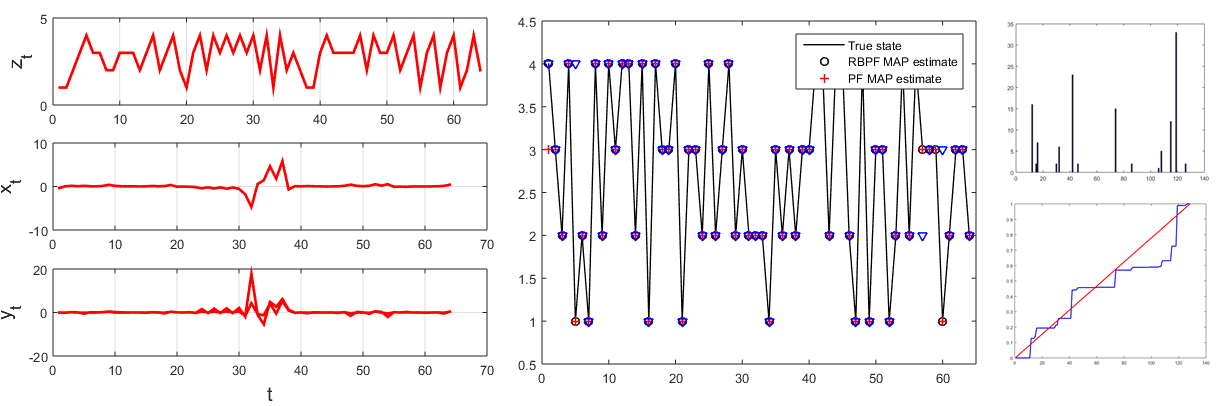
\includegraphics[width=0.9\textwidth, trim={10 10 10 10}]{figures/particle_filter_merged.png}
    \caption{Particle Filter inference using PF and RBPF applied to Switching Linear Dynamic System.}
    \label{fig:pf_merged}
\end{figure}
We can see that the inferred states closely correspond to the ground truth. Also shown is a particle resampling step (right) where only a fraction of the particles survive to the next iteration.


\subsection{Information Theory}

Information theory addresses the problems of data representation and reliable transmission of information. In order to measure information content, we define several information measures below.

\subsubsection{Entropy}

The entropy of a random variable is a measure of its uncertainty. Let $X$ be a discrete random variable with probability mass function $p(x)$, then its entropy is defined as:
\begin{equation}
    H(X) = -\sum_{x} p(x) \log p(x) = -E[\log p(x)]
\end{equation}
A maximum entropy discrete distribution is the uniform distribution. For a random variable with support $K$ and $p(x)=1/K$, the entropy is $H(X)= -\sum \frac{1}{K} \log \frac{1}{K} = \log_2 K$. Thus, entropy is measured in bits (using log base 2) or nats (using log base $e$). In contrast, the entropy of a deterministic random variable with $p(x) = \delta[x]$ is $H(X) = 1\log 1 = 0$. In the special case of a binary random variable $X \in \{0,1\}$ with $p(x=1)=p$, the entropy is
\begin{equation}
    H(X) = -p \log p - (1-p)\log (1-p)
\end{equation}
It is a concave function with maximum uncertainty of $1$ bit occuring at $p=\frac{1}{2}$, when $p=0$ or $p=1$, the entropy is $0$. Since entropy is a concave function on the space of distributions, we have:
\begin{equation}
    H(\lambda p_1 + (1-\lambda) p_2) \geq \lambda H(p_1) + (1-\lambda) H(p_2)
\end{equation}
Since $0\leq p(x) \leq 1$, we have $\log \frac{1}{p(x)} \geq 0$, and for a discrete $X$, the entropy is non-negative: $H(X)\geq 0$. We can find an upper bound for entropy using the Jensen's inequality:
\begin{eqnarray}
    H(X) &=& \sum_{x \in \cal X} p(x)\log \frac{1}{p(x)} \\
         &\leq& \log \sum_{x \in \cal X} p(x)\times \frac{1}{p(x)} \\
         &=& \log \sum_{x \in \cal X} 1 \\
         &=& \log |\cal X|
\end{eqnarray}
We also note that entropy is independent of permutation or cyclical shifts of the support of our distribution, i.e. it only depends on the point masses $p(x)$.\\

The joint entropy of a pair of discrete random variables $X$ and $Y$ is defined as:
\begin{equation}
    H(X,Y) = -\sum_x \sum_y p(x,y) \log p(x,y) = -E[\log p(x,y)]
\end{equation}
when two variables are independent the joint entropy is additivie: $H(X,Y) = H(X) + H(Y)$ iff $p(x,y) = p(x)p(y)$. The conditional entropy is defined as:
\begin{eqnarray}
    H(X|Y) &=& \sum_y p(y)H(X|Y=y) = -\sum_y p(y)\sum_x p(x|y)\log p(x|y) \\
           &=& -\sum_x \sum_y p(x,y)\log p(x|y) = -E[\log p(x|y)]
\end{eqnarray}
Note that conditioning on $Y$ the uncertainty over $X$ reduces on average: $H(X|Y) \leq H(X)$. The entropy of a pair of variables follows the chain rule:
\begin{eqnarray}
    H(X,Y) = H(X) + H(Y|X) = H(Y) + H(X|Y)
\end{eqnarray}
which follows from the chain rule for probability: $p(x,y) = p(x)p(y|x) = p(y)p(x|y)$. The chain rule can be generalized for multiple random variables $X_1,...,X_N$:
\begin{equation}
    H(X_1,...,X_N) = \sum_{i=2}^{N}H(X_i|X_1,...,X_{i-1}) + H(X_1) \leq \sum_{i=1}^{N} H(X_i)
\end{equation}
where the inequality follows from the fact that conditioning reduces entropy. For continuous random variables, the multivariate Gaussian is the distribution with maximum differential entropy:
\begin{eqnarray}
    h(X_1,...,X_N) &=& \int p(x) \log \frac{1}{p(x)} dx \\
    &=& \int p(x) \bigg[\frac{1}{2}\log (2\pi)^{d}|\Sigma| + \frac{1}{2}(x-\mu)^{T}\Sigma^{-1}(x-\mu)\bigg] dx \\
    &=& \frac{1}{2}\log (2\pi)^{d}|\Sigma| + \frac{1}{2}E[(x-\mu)^{T}\Sigma^{-1}(x-\mu)] \\
    &=& \frac{1}{2}\log (2\pi)^{d}|\Sigma| + \frac{1}{2}Tr\{\Sigma^{-1}\Sigma\} \\
    &=& \frac{1}{2}\log (2\pi)^{d}|\Sigma| + \frac{1}{2}d \log e = \frac{1}{2}\log\big[(2\pi e)^d|\Sigma|\big] 
\end{eqnarray}
In information theory, the analog of the law of large numbers is the Asymptotic Equipartition Property (AEP). The AEP states that:
\begin{theorem}
(AEP) If $X_1$,$X_2$,...,$X_n$ are iid $\sim p(x)$ then
\begin{equation}
    -\frac{1}{n} \log p(X_1, X_2,...,X_n) \rightarrow H(X) ~~~\mathrm{in~probability}
\end{equation}
\end{theorem}
\textit{Proof}.
\begin{equation}
    -\frac{1}{n}\log p(X_1, X_2,...,X_n) = -\frac{1}{n}\sum_i \log p(X_i) \rightarrow -E[\log p(X)] = H(X)
\end{equation}
Thus, the probability $p(X_1,...,X_n)$ assigned to an observed sequence will be close to $2^{-nH(X)}$. This enables us to classify the set of all sequences into a typical set, where the sample entropy is close to the true entropy and the nontypical set that contains all other sequences. 

\subsubsection{KL divergence}

One way to measure the similarity between two probability distributions $p(x)$ and $q(x)$ is the Kullback-Leibler divergence or relative entropy. It is defined as follows:
\begin{equation}
    KL(p||q) = \sum_x p(x) \log \frac{p(x)}{q(x)}
\end{equation}
we can re-write it as:
\begin{equation}
    KL(p||q) = \sum_x p(x)\log p(x) - \sum_x p(x)\log q(x) = -H(p) + H(p,q)
\end{equation}
where $H(p,q)$ is the cross-entropy. The regular entropy can be written as $H(p,p)$ and therefore KL divergence can be seen as a penalty of extra bits needed to encode the data due to the fact that we used a distribution $q(x)$ to represent the data instead of the true distribution $p(x)$. 
\begin{theorem}
 (Information Inequality) $KL(p||q)\geq 0$ with equality iff $p = q$. 
\end{theorem}
\textit{Proof}.
\begin{eqnarray}
    -KL(p||q) &=& -\sum_x p(x) \log \frac{p(x)}{q(x)} = \sum_x p(x)\log \frac{q(x)}{p(x)} \\
              &\leq& \log \sum_x p(x) \frac{q(x)}{p(x)} = \log \sum_x q(x)\\
              &\leq& \log 1 = 0
\end{eqnarray}
where we used the Jensen's inequality, which states that for any convex function $f(x)$, we have
\begin{equation}
    f\bigg(\sum_{i=1}^{n}\lambda_i x_i \bigg) \leq \sum_{i=1}^{n} \lambda_i f(x_i)
\end{equation}
where $\lambda_i \geq 0$ and $\sum_{i=1}^{n}\lambda_i = 1$.
However, KL divergence is not a true distance between distributions because it is not symmetric ($KL(p||q) \neq KL(q||p))$ and it does not satisfy the triangle inequality. We can use the information inequality to derive an upper bound on entropy. Let $u(x) = 1/|\cal X|$ be the uniform distribution, then:
\begin{eqnarray}
    0 &\leq& KL(p||u) = \sum_x p(x)\log \frac{p(x)}{u(x)} \\
      &=& \sum_x p(x)\log p(x) - \sum_x p(x)\log u(x) \\
      &=& -H(X) + \log |\cal X|
\end{eqnarray}
Thus, $H(X) \leq \log |\cal X|$ with equality iff $p(x) = u(x)$. 

\begin{theorem}
   $KL(p||q)$ is convex in the pair $(p,q)$, i.e.
   \begin{equation}
        KL(\lambda p_1 + (1-\lambda)p_2 || \lambda q_1 + (1-\lambda) q_2) \leq \lambda KL(p_1||q_1) + (1-\lambda) KL(p_2||q_2)
   \end{equation}
\end{theorem}
\textit{Proof}. Expanding the inequality above, we want to show that
\begin{eqnarray}
\sum_x(\lambda p_1(x) + (1-\lambda)p_2(x))\log\frac{\lambda p_1(x) + (1-\lambda)p_2(x)}{\lambda q_1(x) + (1-\lambda)q_2(x)} \leq \\
\lambda \sum_x p_1(x)\log\frac{p_1(x)}{q_1(x)} + (1-\lambda)\sum_x p_2(x)\log\frac{p_2(x)}{q_2(x)}
\end{eqnarray}
Then for a fixed $x$, it suffices to show that
\begin{equation}
    \sum_{i=1,2} \lambda_i p_i \log \frac{\lambda_i p_i}{\lambda_i q_i} \geq \bigg(\sum_{i=1,2}\lambda_i p_i \bigg)\bigg(\log \frac{\sum_i \lambda_i p_i}{\sum_i \lambda_i q_i} \bigg)
\end{equation}
where $\lambda_1 = \lambda$ and $\lambda_2 = 1-\lambda$, which is exactly the log-sum inequality.\\

In order to find a distribution $q(x) \in Q$ that is closest to $p(x) \in P$, we can minimize $KL(q||p)$ with respect to $q(x)$ known as I-projection or information projection:
\begin{equation}
    (\mathrm{I-projection}): ~~~ q(x) = \arg \min_{q \in Q} KL(q||p)
\end{equation}
Since the KL divergence is not symmetric in its arguments, the above expression will give different behavior compared to minimizing $KL(p||q)$ known as M-projection or moment projection:
\begin{equation}
    (\mathrm{M-projection}): ~~~ q(x) = \arg \min_{q \in Q} KL(p||q)
\end{equation}
Both the I-projection and the M-projection are projections of a probability distribution $p(x)$ onto a set of distributions $Q$. For I-projection, $q(x)$ will typically under-estimate the support of $p(x)$ and will lock onto one of its modes. This is due to $q(x)=0$ whenever $p(x)=0$ to make sure KL divergence stays finite. For M-projection, $q(x)$ will typically over-estimate the support of $p(x)$ and will cover all of its modes. This is due to $q(x)>0$ whenever $p(x)>0$ to make sure KL divergence stays finite. The I-projection is useful in setting up information geometry because of the following inequality:
\begin{equation}
    KL(q||p) \geq KL(q||p^{\ast}) + KL(p^{\ast}||p)
\end{equation}
The inequality can be interpreted as information-geometric version of Pythagoras' triangle inequality theorem, where KL divergernce is viewed as squared distance in Euclidean space.\\
If we are interested in measuring the distance between two multivariate Gaussian distributions with means $\mu_1$ and $\mu_2$ and covariances $\Sigma_1$ and $\Sigma_2$, the KL divergence can be computed in closed form:
\begin{eqnarray}
    KL(p||q) &=& \int p(x) \log \frac{p(x)}{q(x)} = \int [\log p(x) - \log q(x)] p(x) dx \nonumber \\
    &=& \int \bigg[\frac{1}{2}\log\frac{|\Sigma_2|}{|\Sigma_1|}-\frac{1}{2}(x-\mu_1)^{T}\Sigma_{1}^{-1}(x-\mu_1) + \frac{1}{2}(x-\mu_2)^{T}\Sigma_{2}^{-1}(x-\mu_2)\bigg]p(x) dx \nonumber \\
    &=& \frac{1}{2}\log\frac{|\Sigma_2|}{|\Sigma_1|}-\frac{1}{2}Tr\{E[(x-\mu_1)(x-\mu_1)^{T}\Sigma_{1}^{-1}]\} + \frac{1}{2}E[(x-\mu_2)^{T}\Sigma_{2}^{-1}(x-\mu_2)] \nonumber \\
    &=& \frac{1}{2}\log\frac{|\Sigma_2|}{|\Sigma_1|}-\frac{1}{2}Tr\{I_d\}+\frac{1}{2}(\mu_1-\mu_2)^{T}\Sigma_{2}^{-1}(\mu_1 - \mu_2) + \frac{1}{2}Tr\{\Sigma_{2}^{-1}\Sigma_1\} \nonumber \\
    &=& \frac{1}{2}\bigg[\log\frac{|\Sigma_2|}{|\Sigma_1|}-d+Tr(\Sigma_{2}^{-1}\Sigma_1)+(\mu_2-\mu_1)^{T}\Sigma_{2}^{-1}(\mu_2 - \mu_1) \bigg]
\end{eqnarray}


\subsubsection{Mutual Information}

Mutual information (MI) is a measure of overlap of random variables: amount of information one random variable contains about another random variable. Mutual information measures how similar the joint distribution $p(x,y)$ is compared to the factorized distribution $p(x)p(y)$ when the two variables are independent:
\begin{equation}
    I(X;Y) = KL(p(x,y)||p(x)p(y)) = \sum_x \sum_y p(x,y) \log \frac{p(x,y)}{p(x)p(y)}
\end{equation}
where $I(X;Y)\geq 0$ with equality iff the variables are independent: $p(x,y)=p(x)p(y)$. Mutual information between $X$ and $Y$ can be interpreted as the reduction in uncertainty about $X$ after observing $Y$ or by symmetry, the reduction in uncertainty about $Y$ after observing $X$:
\begin{equation}
    I(X;Y) = H(X) - H(X|Y) = H(Y) - H(Y|X) = H(X) + H(Y) - H(X,Y)
\end{equation}
\begin{figure}[tbhp]
    \centering
    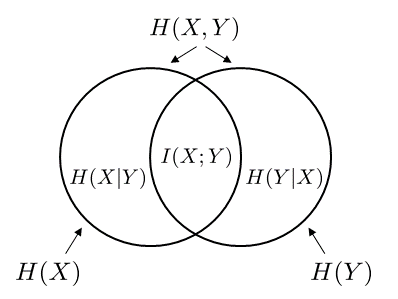
\includegraphics[width=0.4\textwidth, trim={10 10 10 10}]{figures/mutual_info.png}
    \caption{Relationship between entropy and mutual information}
    \label{fig:mutual_info}
\end{figure}
The relationship between entropy and MI is captured in a Venn diagram in Figure \ref{fig:mutual_info}. Note that entropy can be viewed as self-information $H(X) = I(X;X)$. The MI is the expected value of pointwise mutual information:
\begin{equation}
    PMI(x,y) = \log \frac{p(x,y)}{p(x)p(y)} = \log \frac{p(x|y)}{p(x)} = \log \frac{p(y|x)}{p(y)}
\end{equation}
This can be interpreted as the amount we learn from updating the prior $p(x)$ into the posterior $p(y|x)$
\begin{theorem}
(Data Processing Inequality). Let $X$, $Y$, $Z$ form the following Markov chain: $X\rightarrow Y\rightarrow Z$, then the following inequality holds:
\begin{equation}
    I(X;Y) \geq I(X;Z)
\end{equation}
\end{theorem}
\textit{Proof}. By the chain rule, we can expand mutual information in two different ways:
\begin{equation}
    I(X;Y,Z) = I(X;Z) + I(X;Y|Z) = I(X;Y) + I(X;Z|Y)
\end{equation}
Since $X$ is conditionally independent of $Z$ given $Y$, we have $I(X;Z|Y) = 0$ and therefore
\begin{equation}
    I(X;Y) = I(X;Z) + I(X;Y|Z)
\end{equation}
Since $I(X;Y|Z) \geq 0$, we have the inequality: $I(X;Y)\geq I(X;Z)$.
We can use the data processing inequality to show that \textit{sufficient statistics} preserves mutual information. In particular consider the data generating process: $\theta \rightarrow X \rightarrow T(X)$. Given distribution parameters $\theta$, we generate data by sampling from $f_{\theta}(x)$ and then we compute a statistic $T(X)$. The statistic $T(X)$ is called sufficient for $\theta$ if it contains all the information in $X$ about $\theta$, i.e. the data processing inequality is satisfied with equality:
\begin{equation}
    I(\theta; X) = I(\theta; T(X))
\end{equation}
Hence sufficient statistics compresses the information about $\theta$ using sampled data.\\

For a bivariate Gaussian distribution we can compute $I(X;Y)$ as follows.\\
Let $\rho = cov(X,Y)/\sigma_x \sigma_y$, and $\sigma^2 = var(X) = var(Y)$ then $h(X) = h(Y) = \frac{1}{2}\log(2\pi e)\sigma^2$ and
\begin{equation}
    h(X,Y) = \frac{1}{2}\log\big[(2\pi e)^{2}|\Sigma|\big] = \frac{1}{2}\log(2\pi e)^{2}\sigma^4(1-\rho^2)
\end{equation}
Therefore,
\begin{equation}
    I(X;Y) = h(X) + h(Y) - h(X,Y) = -\frac{1}{2}\log (1- \rho^2)
\end{equation}


\subsection{Imbalanced Learning}

Most classification algorithms will only perform optimally when the number of samples in each class is roughly the same. Highly skewed datasets where the minority class is outnumbered by one or more classes commonly occur in fraud detection, medical diagnosis and computational biology. One way of addressing this issue is by re-sampling the dataset to offset the imbalance and arrive at a more robust and accurate decision boundary. Re-sampling techniques can be broadly divided into four categories: undersampling the majority class, over-sampling the minority class, combining over and under sampling, and creating ensemble of balanced datasets \cite{He2009}.\\

\begin{figure}[tbhp]
    \centering
    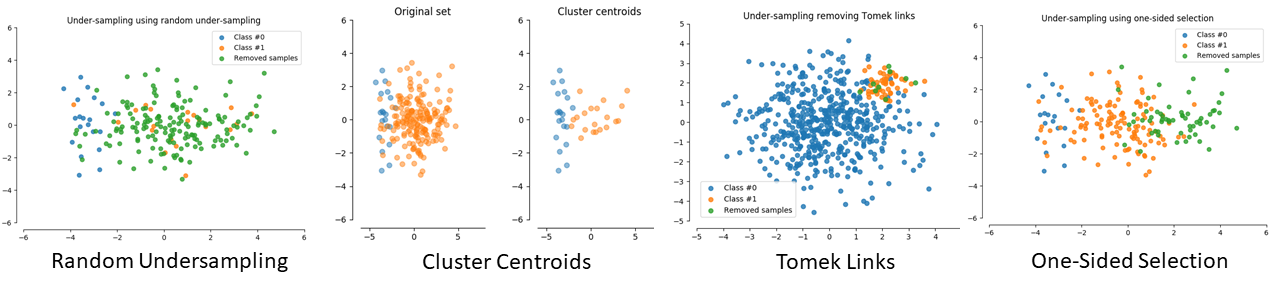
\includegraphics[width=0.95\textwidth, trim={10 10 10 10}]{figures/undersampling.png}
    \caption{Four undersampling strategies: random, cluster centroids, Tomek links, one-sided selection.}
    \label{fig:undersampling}
\end{figure}

\textit{Undersampling strategies}. Undersampling methods remove data from the majority class of the original dataset as shown in Figure \ref{fig:undersampling}. Random Under Sampler simply removes data points from the majority class uniformly at random. Cluster Centroids is a method that replaces cluster of samples by the cluster centroid of a K-means algorithm, where the number of clusters is set by the level of undersampling. Tomek links remove unwanted overlap between classes where Tomek links are removed until all minimally distanced nearest neighbor pairs are of the same class. A Tomek link is defined as follows: given an instance pair $(x_i, x_j)$, where $x_i \in S_{min}$, $x_j \in S_{maj}$ and $d(x_i,x_j)$ is the distance between $x_i$ and $x_j$, then the $(x_i, x_j)$ pair is called a Tomek link if there's no instance $x_k$ such that $d(x_i, x_k) < d(x_i, x_j)$ or $d(x_j, x_k) < d(x_i, x_j)$. In this way, if two instances form a Tomek link then either one of these instances is noise or both are near a border. Therefore one can use Tomek links to clean up overlap between classes. By removing overlapping examples, one can establish well-defined clusters in the training set and lead to improved classification performance. The One Sided Selection (OSS) method selects a representative subset of the majority class $E$ and combines it with the set of all minority examples $S_{min}$ to form $N = \{E\cup S_{min}\}$. The reduced set $N$ is further processed to remove all majority class Tomek links.\\  

\begin{figure}[tbhp]
    \centering
    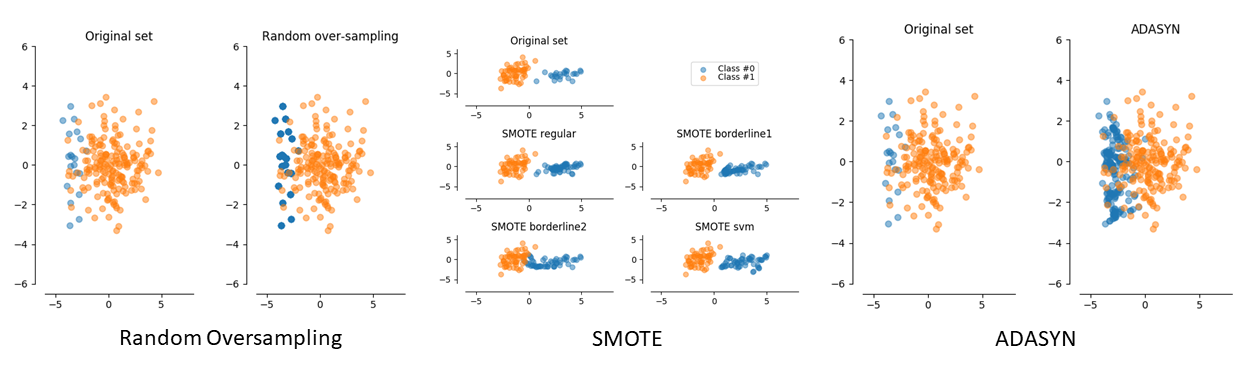
\includegraphics[width=0.95\textwidth, trim={10 10 10 10}]{figures/oversampling.png}
    \caption{Three oversampling strategies: random, SMOTE, ADASYN.}
    \label{fig:oversampling}
\end{figure}

\textit{Oversampling strategies}. Oversampling methods append data to the minority class of the original dataset as shown in Figure \ref{fig:oversampling}. Random Over Sampler simply adds data points to the minority class uniformly at random. Synthetic Minority Oversampling Technique (SMOTE) generates synthetic examples by finding $K$ nearest neighbors in the feature space and generating a new data point along the line segments joining any of the $K$ minority class nearest neighbors. Synthetic samples are generated in the following way: take the difference between the feature vector (sample) under consideration and its nearest neighbor, multiply this difference by a random number between $0$ and $1$ and add it to the feature vector under consideration thus augmenting the dataset with a new data point. Adaptive Synthetic Sampling (ADASYN) uses a weighted distribution for different minority class examples according to their level of difficulty in learning, where more synthetic data is generated for minority class examples that are harder to learn. As a result, the ADASYN approach improves learning of imbalanced dataset in two ways: reducing the bias introduced by class imbalance and adaptively shifting the classification decision boundary toward the difficult examples.\\ 

It's possible to combine over-sampling and under-sampling techniques into a hybrid strategy. Common examples include SMOTE and Tomek links or SMOTE and Edited Nearest Neighbors (ENN). Additional ways of learning on imbalanced datasets include weighing training instances, introducing different misclassification costs for positive and negative examples and bootstrapping. 


\subsection{Ensemble Methods}

Ensemble methods are meta-algorithms that combine several machine learning techniques into one predictive model in order to decrease variance (bagging), bias (boosting), or improve predictions (stacking). Ensemble methods can be divided into two groups: \textit{sequential} ensemble methods where the base learners are generated sequentially (e.g. AdaBoost) and \textit{parallel} ensemble methods where the base learners are generated in parallel (e.g. Random Forest). The basic motivation of sequential methods is to exploit the dependence between the base learners since the overall performance can be boosted by weighing previously mislabeled examples with higher weight.  The basic motivation of parallel methods is to exploit independence between the base learners since the error can be reduced dramatically by averaging.\\  

Most ensemble methods use a single base learning algorithm to produce homogeneous base learners, i.e. learners of the same type leading to \textit{homogeneous ensembles}. There are also some methods that use heterogeneous learners, i.e. learners of different types, leading to \textit{heterogeneous ensembles}. In order for ensemble methods to be more accurate than any of its individual members the base learners have to be as accurate as possible and as diverse as possible. \\

\subsubsection{Bagging}

Bagging stands for bootstrap aggregation. One way to reduce the variance of an estimate is to average together multiple estimates. For example, we can train $M$ different trees $f_m$ on different subsets of the data (chosen randomly with replacement) and compute the ensemble:
\begin{equation}
   f(x) = \frac{1}{M}\sum_{m=1}^{M}f_m(x)
\end{equation}
Bagging uses bootstrap sampling to obtain the data subsets for training the base learners. For aggregating the outputs of base learners, bagging uses voting for classification and averaging for regression.

\begin{figure}[tbhp]
    \centering
    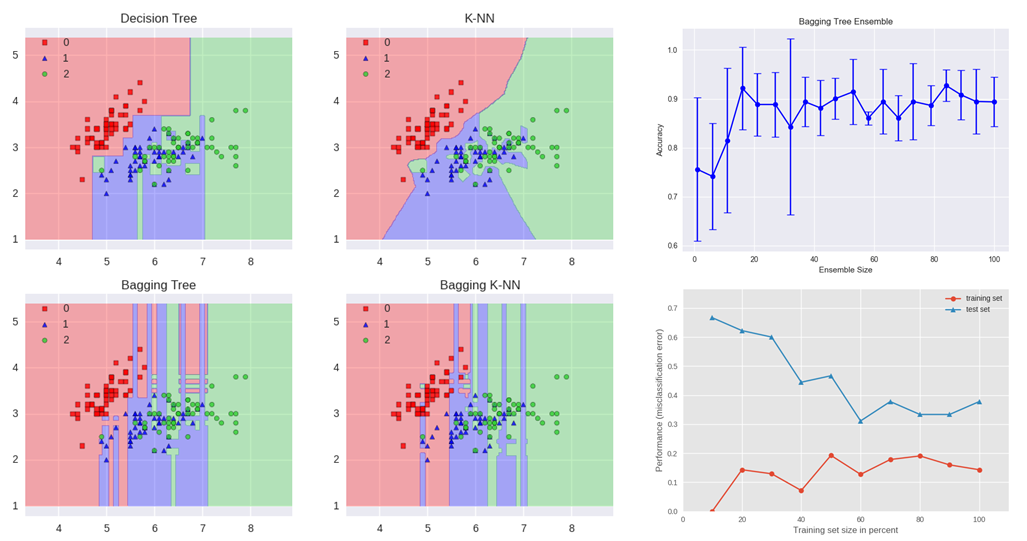
\includegraphics[width=0.95\textwidth, trim={10 10 10 10}]{figures/ensemble_bagging_merged.png}
    \caption{Bagging Ensemble with decision tree and k-NN as base estimator.}
    \label{fig:ensemble_bagging}
\end{figure}

Figure \ref{fig:ensemble_bagging} shows the decision boundary of a decision tree and k-NN classifiers along with their bagging ensembles applied to the Iris dataset. The decision tree shows axes parallel boundaries while the $k=1$ nearest neighbors fits closely to the data points. The bagging ensembles were trained using $10$ base estimators with $0.8$ subsampling of training data and $0.8$ subsampling of features. The decision tree bagging ensemble achieved higher accuracy in comparison to k-NN bagging ensemble because k-NN are less sensitive to perturbation on training samples and therefore they are called \textit{stable learners}. Combining stable learners is less advantageous since the ensemble will not help improve generalization performance. The figure also shows how the test accuracy improves with the size of the ensemble. Based on cross-validation results, we can see the accuracy increases until approximately $20$ base estimators and then plateaus afterwards. Thus, adding base estimators beyond $20$ only increases computational complexity without accuracy gains for the Iris dataset. The figure also shows learning curves for the bagging tree ensemble. We can see an average error of $0.15$ on the training data and a U-shaped error curve for the testing data. The smallest gap between training and test errors occurs at around $80\%$ of the training set size.\\

A commonly used class of ensemble algorithms are forests of randomized trees. In \textbf{random forests}, each tree in the ensemble is built from a sample drawn with replacement (i.e. a bootstrap sample) from the training set. In addition, instead of using all the features, a random subset of features is selected further randomizing the tree. As a result, the bias of the forest increases slightly but due to averaging of less correlated trees, its variance decreases resulting in an overall better model.\\

In \textbf{extremely randomized trees} algorithm randomness goes one step further: the splitting thresholds are randomized. Instead of looking for the most discriminative threshold, thresholds are drawn at random for each candidate feature and the best of these randomly-generated thresholds is picked as the splitting rule. This usually allows to reduce the variance of the model a bit more, at the expense of a slightly greater increase in bias.\\  


\subsubsection{Boosting}

Boosting refers to a family of algorithms that are able to convert weak learners to strong learners. The main principle of boosting is to fit a sequence of weak learners (models that are only slightly better than random guessing, such as small decision trees) to weighted versions of the data, where more weight is given to examples that were mis-classified by earlier rounds. The predictions are then combined through a weighted majority vote (classification) or a weighted sum (regression) to produce the final prediction. The principal difference between boosting and the committee methods such as bagging is that base learners are trained in sequence on a weighted version of the data.   

Algorithm \ref{alg:adaboost} describes the most widely used form of boosting algorithm called \textbf{AdaBoost} which stands for adaptive boosting \cite{Freund97}. 

\begin{algorithm}
\caption{AdaBoost}
\label{alg:adaboost}
\begin{algorithmic}[1]
\STATE Init data weights $\{w_n\}$ to $1/N$ 
\STATE \textbf{for} $m = 1$ to $M$ \textbf{do}  
\STATE ~~~ fit a classifier $y_m(x)$ by minimizing weighted error function $J_m$:
\STATE ~~~ $J_m = \sum_{n=1}^{N} w_{n}^{(m)}1[y_m(x_n) \neq t_n]$
\STATE ~~~ compute $\epsilon_m = \sum_{n=1}^{N} w_{n}^{(m)}1[y_m(x_n) \neq t_n] / \sum_{n=1}^{N}w_{n}^{(m)}$
\STATE ~~~ evaluate $\alpha_m = \log \big(\frac{1-\epsilon_m}{\epsilon_m}\big)$
\STATE ~~~ update the data weights: $w_{n}^{(m+1)} = w_{n}^{(m)}\exp\{\alpha_m 1[y_m(x_n) \neq t_n]\}$
\STATE \textbf{end for}
\STATE Make predictions using the final model: $Y_M(x)=\mathrm{sign}\bigg(\sum_{m=1}^{M}\alpha_m y_m(x)\bigg)$ 
\end{algorithmic}
\end{algorithm}

We see that the first base classifier $y_1(x)$ is trained using weighting coefficients $w_{n}^{(1)}$ that are all equal. In subsequent boosting rounds, the weighting coefficients $w_{n}^{(m)}$ are increased for data points that are misclassified and decreased for data points that are correctly classified. The quantity $\epsilon_m$ represents a weighted error rate of each of the base classifiers. Therefore, the weighting coefficients $\alpha_m$ give greater weight to the more accurate classifiers.\\

\begin{figure}[tbhp]
    \centering
    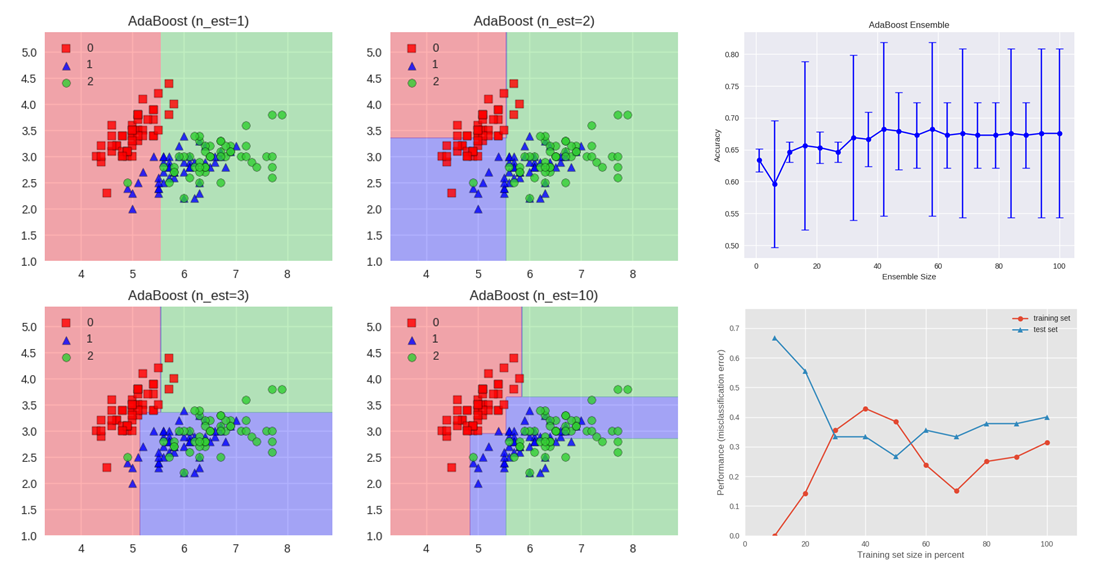
\includegraphics[width=0.95\textwidth, trim={10 10 10 10}]{figures/ensemble_boosting_merged.png}
    \caption{Boosting Ensemble with decision tree as base estimator.}
    \label{fig:ensemble_boosting}
\end{figure}

The AdaBoost algorithm is illustrated in Figure \ref{fig:ensemble_boosting}. Each base learner consists of a decision tree with depth $1$, thus classifying the data based on a feature threshold that partitions the space into two regions separated by a linear decision surface that is parallel to one of the axes. The figure also shows how the test accuracy improves with the size of the ensemble and the learning curves for training and testing data.\\

\textbf{Gradient Tree Boosting} is a generalization of boosting to arbitrary differentiable loss functions. It can be used for both regression and classification problems. Gradient Boosting builds the model in a sequential way:
\begin{equation}
    F_m(x) = F_{m-1}(x) + \gamma_m h_m(x)
\end{equation}
At each stage the decision tree $h_m(x)$ is chosen to minimize a loss function $L$ given the current model $F_{m-1}(x)$:
\begin{equation}
    F_m(x) = F_{m-1}(x) + \arg \min_h \sum_{i=1}^{n} L(y_i, F_{m-1}(x_i) + h(x_i))
\end{equation}
Gradient Boosting attempts to solve this minimization problem numerically via steepest descent. The steepest descent direction is the negative gradient of the loss function evaluated at the current model $F_{m-1}$:
\begin{equation}
    F_m(x) = F_{m-1}(x) + \gamma_m \sum_{i=1}^{n} \nabla_F L(y_i, F_{m-1}(x_i))
\end{equation}
where the step size $\gamma_m$ is chosen using line search. The algorithms for regression and classification differ in the type of loss function used.


\subsubsection{Stacking}

Stacking is an ensemble learning technique that combines multiple classification or regression models via a meta-classifier or a meta-regressor. The base level models are trained based on complete training set then the meta-model is trained on the outputs of base level model as features. The base level often consists of different learning algorithms and therefore stacking ensembles are often heterogeneous. Algorithm \ref{alg:ensemble_stacking} summarizes stacking. 

\begin{algorithm}
\caption{Stacking}
\label{alg:ensemble_stacking}
\begin{algorithmic}[1]
\STATE Input: training data $D=\{x_i,y_i\}_{i=1}^{m}$
\STATE Ouput: ensemble classifier $H$
\STATE \textit{Step 1: learn base-level classifiers}
\STATE \textbf{for} $t = 1$ to $T$ \textbf{do}  
\STATE ~~~ learn $h_t$ based on $D$
\STATE \textbf{end for} 
\STATE \textit{Step 2: construct new data set of predictions}
\STATE \textbf{for} $i = 1$ to $m$ \textbf{do} 
\STATE ~~~ $D_{h} = \{x_{i}^{\prime}, y_i\}$, where $x_{i}^{\prime}=\{h_1(x_i),...,h_T(x_i)\}$
\STATE \textbf{end for}
\STATE \textit{Step 3: learn a meta-classifier}
\STATE learn $H$ based on $D_h$
\STATE return $H$
\end{algorithmic}
\end{algorithm}


\begin{figure}[tbhp]
    \centering
    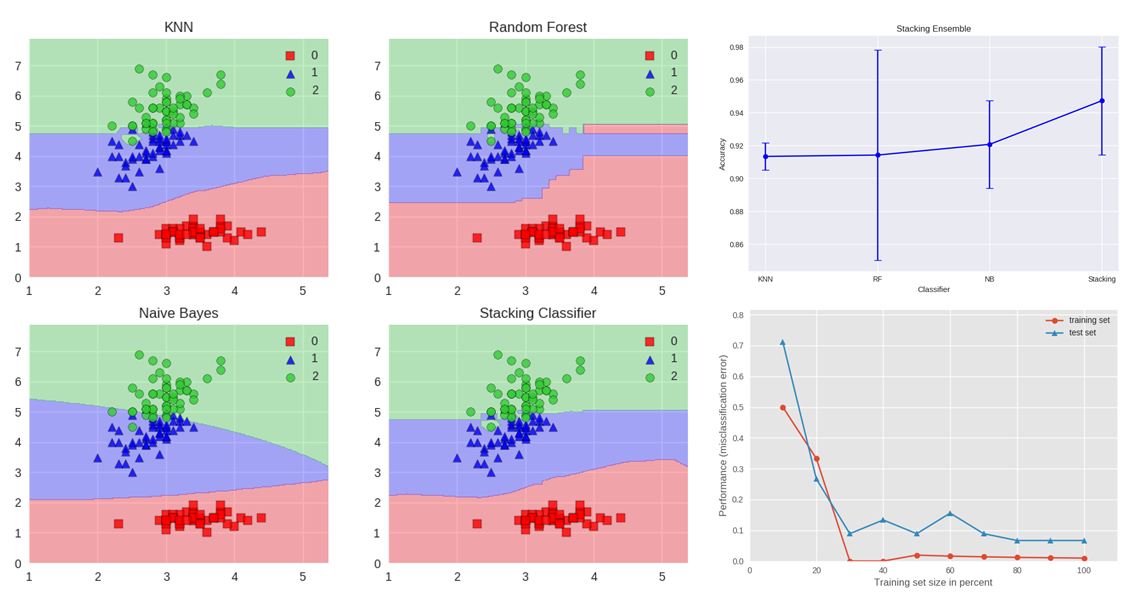
\includegraphics[width=0.95\textwidth, trim={10 10 10 10}]{figures/ensemble_stacking_merged.png}
    \caption{Stacking Ensemble with Logistic Regression as meta-classifier.}
    \label{fig:ensemble_stacking}
\end{figure}

The stacking ensemble is illustrated in Figure \ref{fig:ensemble_stacking}. It consists of k-NN, Random Forest and Naive Bayes base classifiers whose predictions are combined by Lostic Regression as a meta-classifier. We can see the blending of decision boundaries achieved by the stacking classifier. The figure also shows that stacking achieves higher accuracy than individual classifiers and based on learning curves, it shows no signs of overfitting.\\ 





